\documentclass[12pt]{article}   	

% Document Formatting Packages
\usepackage{geometry}            		
\geometry{letterpaper}  
\usepackage[usenames,dvipsnames,svgnames,table]{xcolor}


% Document Navigation Packages
\usepackage[parfill]{parskip}          
\usepackage{enumitem}         

% Math Typesetting Tools
\usepackage{amssymb}
\usepackage{amsmath,mathtools}
\usepackage{framed}

% Hyperref
\usepackage[colorlinks=true,linkcolor=blue,citecolor=red]{hyperref}

% Chemistry Typesetting Tools
\usepackage{mhchem}

% Inserting Figures
\usepackage{graphicx}
\usepackage[section]{placeins}
\graphicspath{ {images/} }			

% Miscellaneous Symbol Packages
\usepackage{textcomp}  		
\usepackage{siunitx}
\usepackage{gensymb}

% Set Document Dimensions
\oddsidemargin = 0in
\topmargin = 0in
\headheight=0pt
\headsep = 0pt
\textheight = 9in
\textwidth = 6.5in
\marginparsep = 0in
\marginparwidth = 0in
\footskip = 18pt
\parindent=15pt
\parskip=0pt

% Title
\title{Weekly Update - Week of 29 April 2018}
\author{Joseph Lucero}
\date{\today}

\begin{document}
\maketitle

%\section*{Color Coding Guide}
%
%Guide to color coding in these updates:
%\begin{itemize}
%	\item \textcolor{Red}{Text in red are points that I really want to emphasize and would like your immediate input on as these are either major hurdles that I am currently facing, or important that I get right to ensure that analysis later on is not affected}
%	\item \textcolor{ForestGreen}{Text in green are questions that are outstanding that I have not been able to find an answer for, but unlike the text in red these questions these questions are not currently hindering me from progressing forward}
%	\item \textcolor{RoyalPurple}{Text in purple are things I just want to stand out apart from my explanations. Thus, things like variable names and major advancements will be colored this way}
%\end{itemize}
%For your convenience, please feel free to skip most of the text (as it is mostly for me to keep track of progress anyways) but if you could kindly look at what I have highlighted I would greatly appreciate it. Thanks!

\section{Past Week}

This \textbf{past week} I was primarily working on \textbf{three} things:

\begin{enumerate}
	\item \textbf{Getting my workstation set up and running}
	\begin{itemize}
		\item The following installations that are worth mentioning were made on the local machine:
		\begin{enumerate}
			\item Homebrew: package manager for Apple computers that allow one to access software necessary to do scientific computing
			\item MacTex: distribution allowing macOS devices to compile \LaTeX code
			\item Visual Studio Code and TeXstudio: Text editors that facilitate coding with shortcuts and fancy syntax highlighting and completions. For Python/C++ code and \LaTeX code, respectively.
			\item iTerm2: a better terminal for macOS that is much more customizable and has better shortcuts and integration
			\item Anaconda: scientific Python distribution that comes with its own package manager. Facilitates scientific computing by coming with the most commonly used packages for scientific computing in Python and also provides its own editor (Spyder) that is good for analysis of numerical outputs.
			\item SourceTree: a GUI for git. Makes it easier to visually see what is going on when working to push changes
			\item XQuartz and xmgrace: Allows for the X11 tunneling and functioning of egs\_view and 3D Dose tools from the cluster on the local machine
			\end{enumerate}
		\item Set up my own home area on the cluster and got it ready for computing
		\begin{itemize}
			\item Installed EGSnrc with egs\_brachy
			\item Completed a working .cshrc file that allows for ease of navigation as well as has aliases, previously defined, that make using the cluster much easier
			\item Compiled egs\_view and got it to communicate with the local workstation
		\end{itemize}
	\end{itemize}
	\item \textbf{Exploring the examples given in the egs\_brachy user code}
	\begin{itemize}
		\item Looked at the different examples to see how egs\_brachy codes work 
		\item Performed an experiment to see what happens when the padding on the outside of the scoring phantom is removed
		\item Intuitively would think that removing the outside padding would result in a lower dosage on the scoring phantom as backscatter events from the surrounding media would be lost if the surrounding media were to be removed.
		\item Worked with the example file ``ex\_prostate\_permanent\_implant.egsinp'' and simply changed the final simulation geometry or the geometry of the surrounding box
		\item Figure~\ref{fig:dose_histogram} shows the dose volume histograms for 3 different configurations
		\begin{itemize}
			\item As we can see for this histogram, removing the padding clearly results in the lowering of the average dose. 
		\end{itemize}
		\item Figure~\ref{fig:cumulative_dose_histogram} shows the cumulative dose volume histogram for the 3 different configurations
	\end{itemize}
	\item \textbf{Reading on fundamentals of radiation dosimetry}
	\begin{itemize}
		\item Finished Chapters 1-6 of Mayes, Nahum \& Rosenwald's \underline{Handbook of Radiotherapy Physics}
		\item Of particular interest to me from this reading that I learned are the following:
		\begin{itemize}
			\item Different interactions of charged particles with matter including elastic scattering and brehmmstrahlung
			\item Concept of stopping power and its relation to the so-called ``Continuous \\ Slowing Down Approximation (CSDA)''
			\item Learned about mass energy abosorption coefficients $ \frac{\mu_{\rm en}}{\rho} $ and their relation to mass attenuation coefficients
			\item Different interactions of radiation (light) with matter including photoelectric effect, Compton effect, pair/triplet production, and coherent scattering
			\item Relation of fluence (particle and energy) to kerma; relation of kerma to dose; relation of fluence to dose
			\item Concept of ``Charged Particle Equilibrium (CPE)'' and how it is able to directly relate dose to collision kerma
		\end{itemize}
	\end{itemize}
	\item \textbf{Read Lymperopoulou \textit{et al}. (2004)}
	\begin{itemize}
		\item Got a basic idea of what the geometry is of the applicator that they are using 
		\item Gives me a starting point for specifying the geometry on egs\_brachy
		\item Also gives good tests to subject the applicator to (eg. changing internal structure and materials of the applicator)
		\item Gives results plots that I can work towards replicating using egs\_brachy		
	\end{itemize}
\end{enumerate}

\section{Next Week}

In the \textbf{next week} I plan on tackling the following \textbf{four} things:

\begin{enumerate}
	\item \textbf{Read about fundamentals of brachytherapy}
	\begin{itemize}
		\item I will primarily be reading Chapter 50 \& 53 of the Handbook
	\end{itemize}
	\item \textbf{Read about the relevant statistics in use in dosimetry}
	\begin{itemize}
		\item I currently know of dose volume histograms, and cumulative dose volume histograms
		\item I will skim the Handbook for any more statistics that are useful 
	\end{itemize}
	\item \textbf{Read the paper by Ma \textit{et al}. (2017)}
	\begin{itemize}
		\item Read this to try and learn more about the origin of the example of HDR therapy with applicator given in egs\_brachy
		\item Also read this to try and figure out what considerations need to be made when designing the applicator
	\end{itemize}
	\item \textbf{Start working on creating the geometry for the applicator in Lymperopoulou \textit{et al}. (2004)}
	\begin{itemize}
		\item Use the geometry given in the TG186 folder of egs\_brachy as a template to begin constructing the applicator
	\end{itemize}
	\item \textbf{(Extra Credit) Run initial simulation on prototype geometry}	
\end{enumerate}

\section{Figures}

\begin{figure}[!ht]
	\centering
	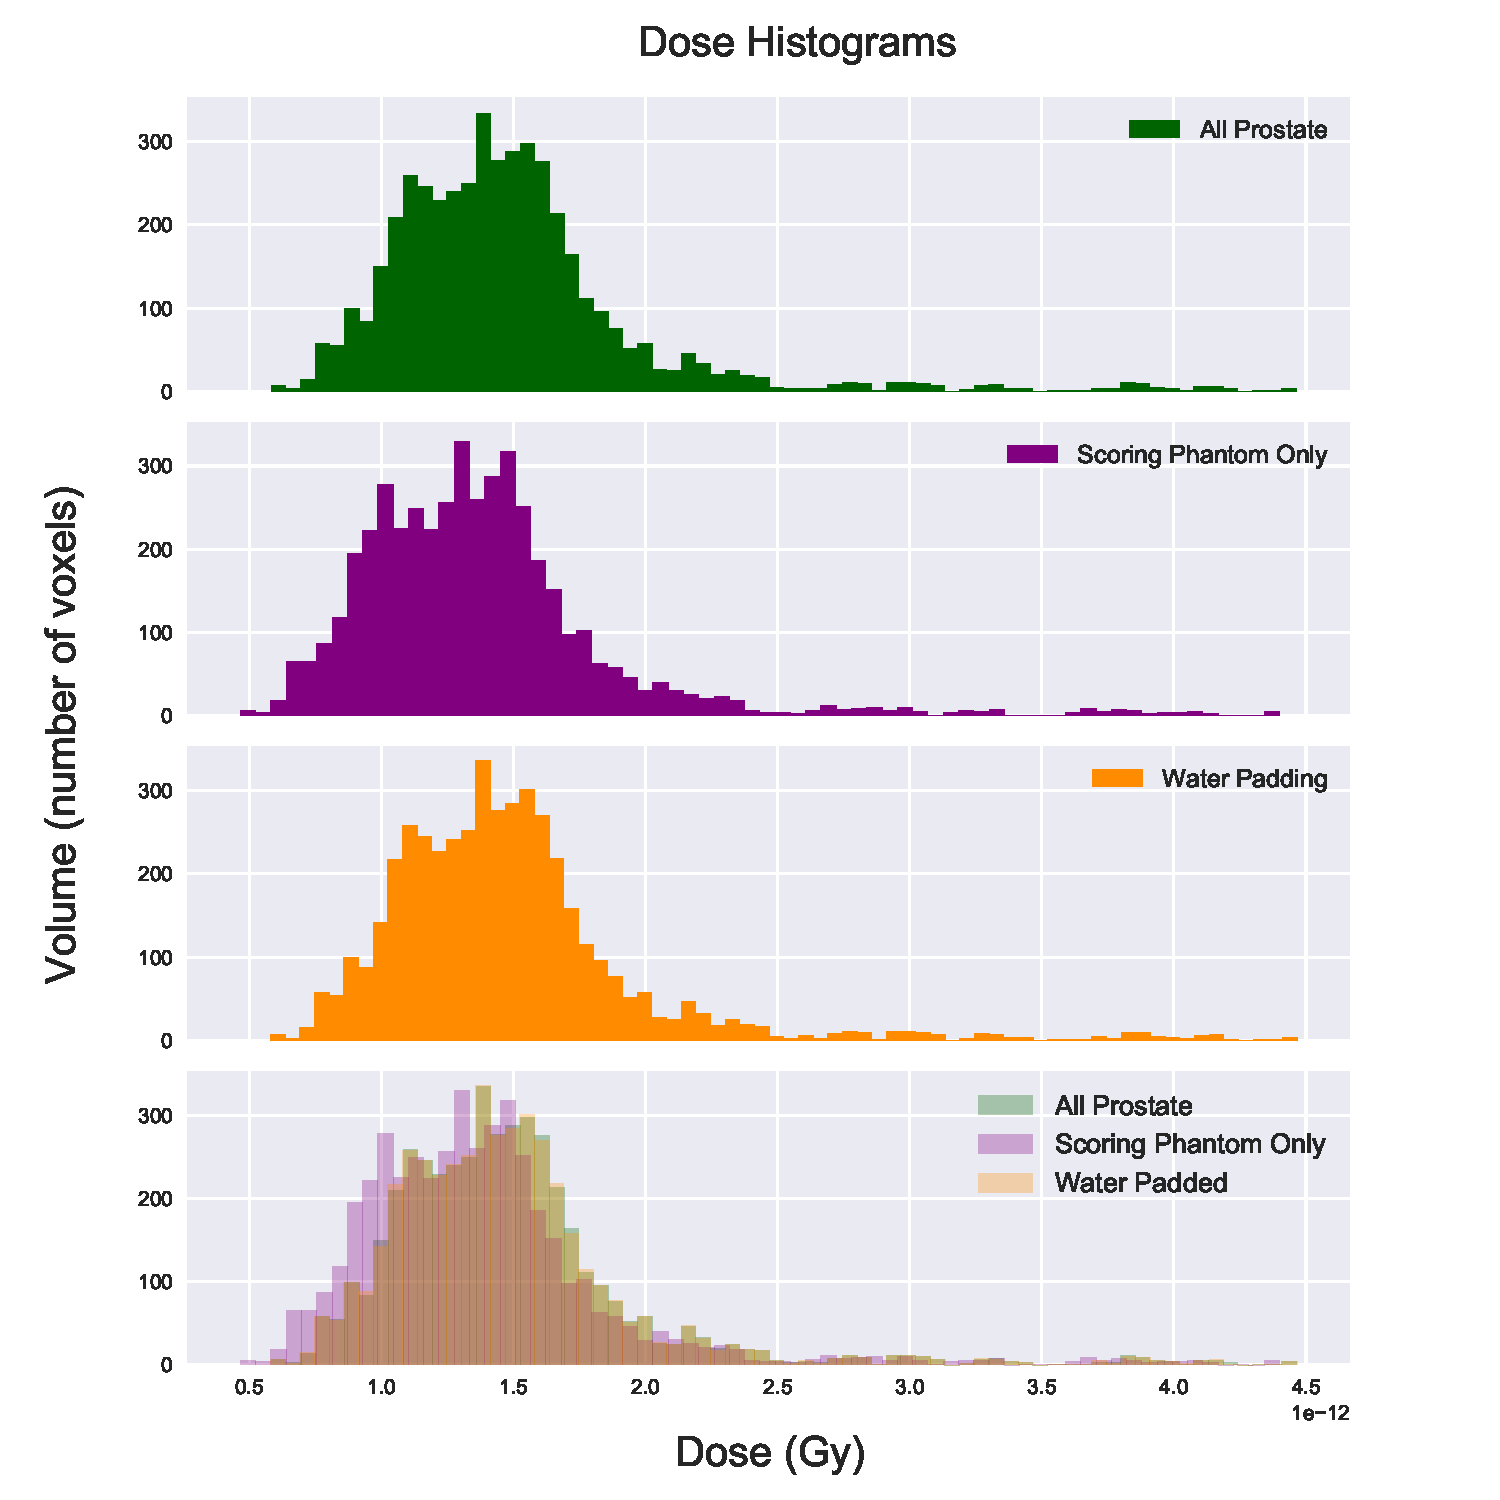
\includegraphics[scale=0.43]{dose_histogram}  
	\caption{Volumetric Dose Histogram (VDH) for various simulation configurations. Top most subplot is for a simulation where both the scoring phantom and the padding surrounding it are made of prostate. The second subplot is for a simulation with no padding and only considering the scoring phantom as the simulation geometry. The third subplot is if scoring phantom is still made of prostate but now padded with water instead. The last subplot is the three subplots above superimposed on one another. Between the results, only the configuration of the geometries were changed. Other parameters were left the same across the different simulations.}
	\label{fig:dose_histogram}
\end{figure}

\begin{figure}[!ht]
	\centering
	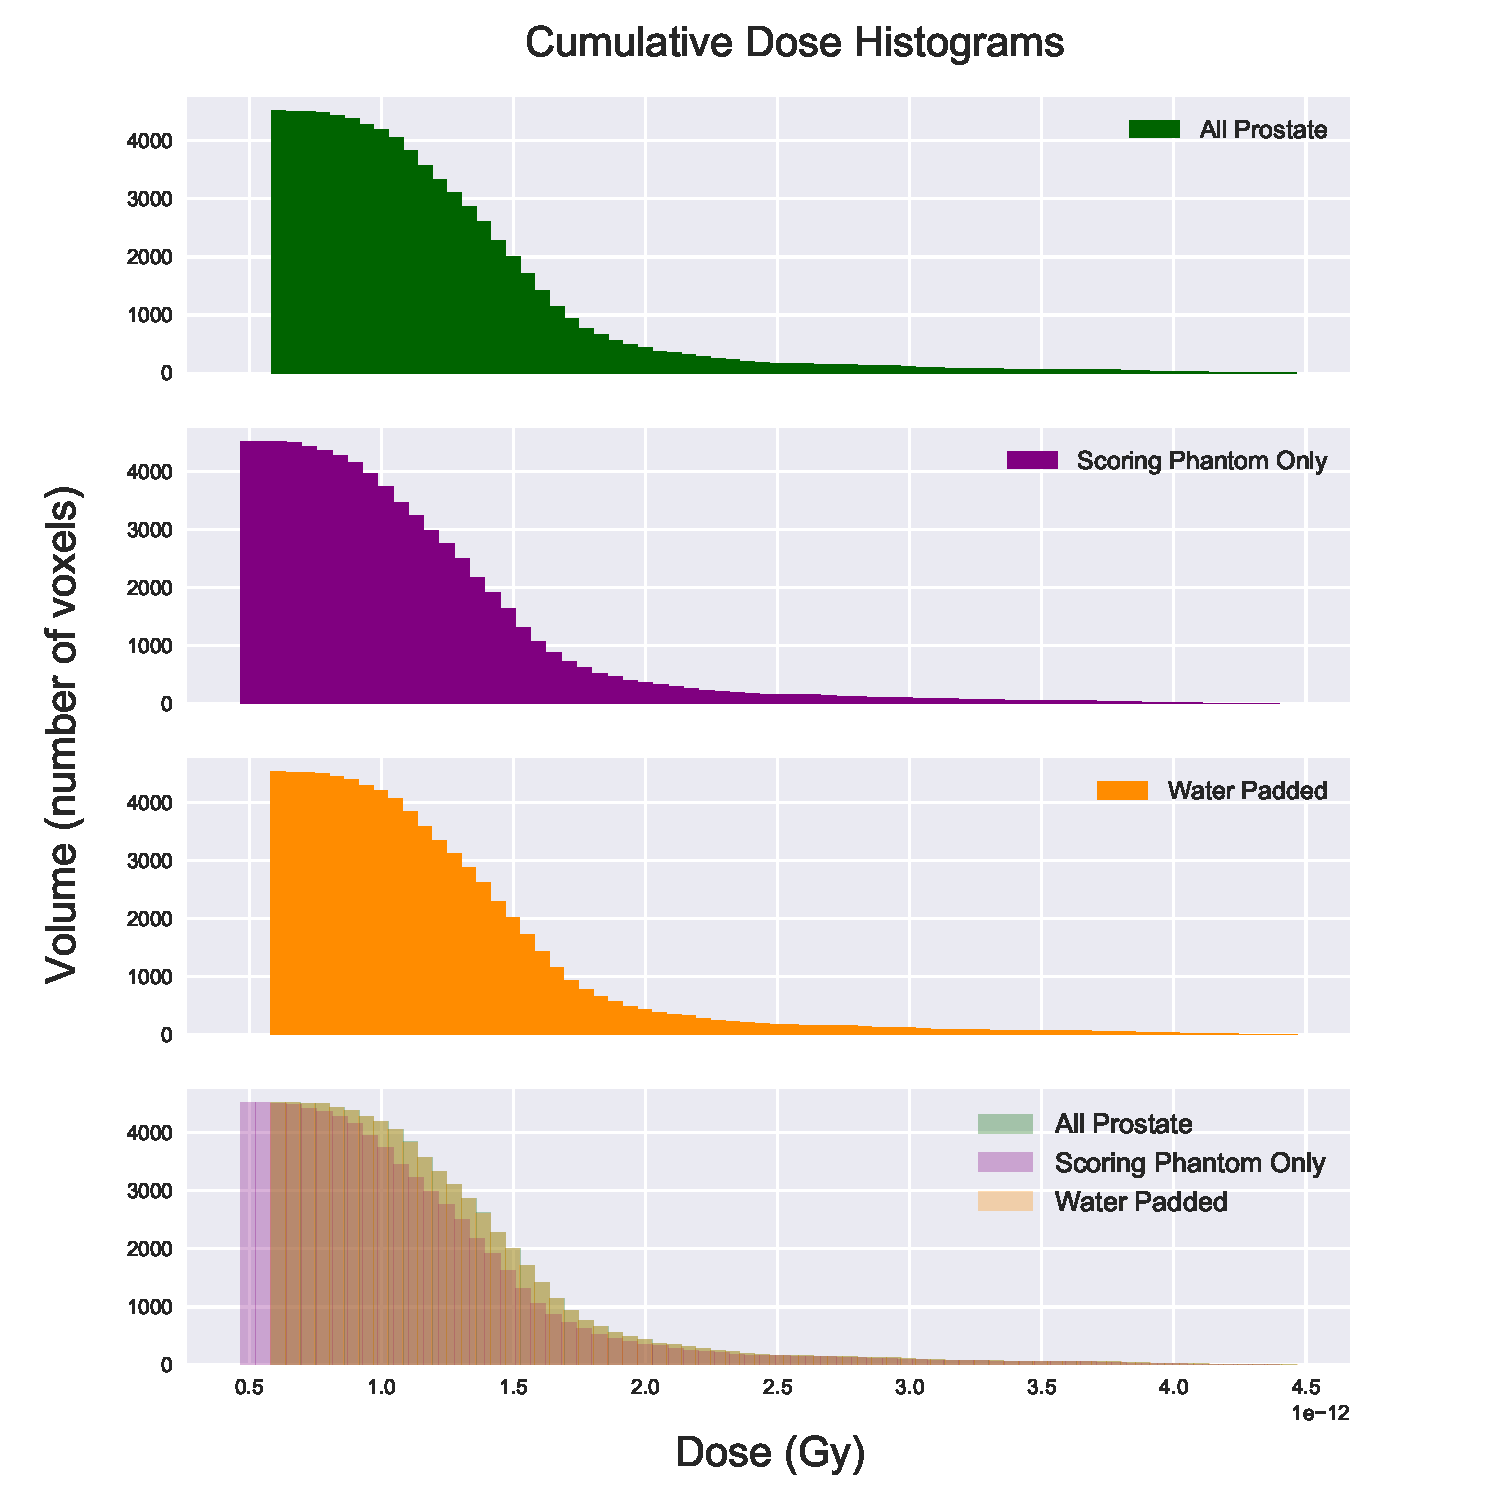
\includegraphics[scale=0.5]{cum_dose_histogram}  
	\caption{Cumulative Volumetric Dose Histogram (VDH) for various simulation configurations. Same configuration for subplots as Fig.~\ref{fig:dose_histogram}}
	\label{fig:cumulative_dose_histogram}
\end{figure}

\end{document}